\documentclass[12pt]{scrreprt} 
\usepackage{graphicx}
\usepackage{tikz}
\usepackage{mathtools}
\usepackage{caption}
\captionsetup[figure]{labelformat=empty}
\usetikzlibrary{automata,positioning}
\PassOptionsToPackage{usenames,dvipsnames,svgnames}{xcolor}


\begin{document} 

\begin{titlepage}

\newcommand{\HRule}{\rule{\linewidth}{0.5mm}} % Defines a new command for the horizontal lines, change thickness here

\center % Center everything on the page

%----------------------------------------------------------------------------------------
%	HEADING SECTIONS
%----------------------------------------------------------------------------------------

\textsc{\LARGE University of North Alabama}\\[1.5cm] % Name of your university/college
\textsc{\Large Programming Languages}\\[0.5cm] % Major heading such as course name

%----------------------------------------------------------------------------------------
%	TITLE SECTION
%----------------------------------------------------------------------------------------

\HRule \\[0.4cm]
{ \huge \bfseries JavaScript}\\[0.4cm] % Title of your document
\HRule \\[1.5cm]
 
%----------------------------------------------------------------------------------------
%	AUTHOR SECTION
%----------------------------------------------------------------------------------------

\begin{minipage}{0.4\textwidth}
\begin{flushleft} \large
\emph{Author:}\\
Jeffrey \textsc{Allen}
\end{flushleft}
\end{minipage}
~
\begin{minipage}{0.4\textwidth}
\begin{flushright} \large
\emph{Professor:} \\
Dr. Patricia \textsc{Roden}
\end{flushright}
\end{minipage}\\[4cm]

{\large \today}\\[3cm] % Date, change the \today to a set date if you want to be precise

\vfill % Fill the rest of the page with whitespace

\end{titlepage}

\tableofcontents 

\chapter{History}

\section{Brendan Eich}

\section{Developer Communities}

% \begin{figure}[h]
	
% 	\centering
% 		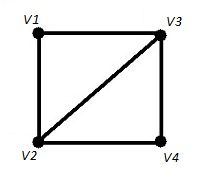
\includegraphics[width=0.25\textwidth]{figure1}
% 	\caption{Figure 1}

% \end{figure}

% \section{Adjacency matrix for $A$} 

% \[ A = \left( \begin{array}{cccc}
% 0 & 1 & 1 & 0 \\
% 1 & 0 & 1 & 1 \\
% 1 & 1 & 0 & 1 \\
% 0 & 1 & 1 & 0 \end{array} \right)\] 

% \section{$A^2$ and $A^3$}

% \[ A^2 = \left( \begin{array}{cccc}
% 2 & 1 & 1 & 2 \\
% 1 & 3 & 2 & 1 \\
% 1 & 2 & 3 & 1 \\
% 2 & 1 & 1 & 2 \end{array} \right)\] 

% \[ A^3 = \left( \begin{array}{cccc}
% 2 & 5 & 5 & 2 \\
% 5 & 4 & 5 & 5 \\
% 5 & 5 & 4 & 5 \\
% 2 & 5 & 5 & 2 \end{array} \right)\] 

% \pagebreak

% \subsection{What values in $A^n$ tell about the graph in Figure 1 & proving your claim for $A^2$} 

% The $n$ in the expression $A^n$ represents the amount of edges that must be used in order to travel between one  node, to another.
% The adjacency matrix for $A^1$ represents $0$ paths between $V_1$ and itself. In the adjacency matrix $A^2$, there are
% $2$ possible paths from $V_1$ to itself utilizing 2 edges.

% \section{Compute the eigenvalues and eigenvectors for $A$}

%   \begin{center}
%   \textbf{Eigenvalues}
%   \end{center}

%   \begin{center}
%   \begin{tabular}{ c c c p{5cm} }
%     $\lambda_1$ & $\rightarrow$ & $\frac{1}{2}(1+\sqrt{17})$ \\        
%     $\lambda_2$ & $\rightarrow$ & $\frac{1}{2}(1-\sqrt{17})$ \\
%     $\lambda_3$ & $\rightarrow$ & -1 \\
%     $\lambda_4$ & $\rightarrow$ & 0 \\
%   \end{tabular}
%   \end{center}

%   \begin{center}
%   \textbf{Eigenvectors}
%   \end{center}

%   \begin{center}
%   $\vec{x}_1 = \begin{pmatrix}1\\\frac{1}{4}(1 + \sqrt{17})\\\frac{1}{4}(1 + \sqrt{17})\\1\end{pmatrix}$
%   $\vec{x}_2 = \begin{pmatrix}1\\\frac{1}{4}(1 - \sqrt{17})\\\frac{1}{4}(1 - \sqrt{17})\\1\end{pmatrix}$
%   $\vec{x}_3 = \begin{pmatrix}0\\-1\\1\\0\end{pmatrix}$
%   $\vec{x}_4 = \begin{pmatrix}-1\\0\\0\\1\end{pmatrix}$
%   \end{center}

% \subsection{Importance of eigenvalues and eigenvectors to graph}

% We observed that there is one zero, one positive, and two negative eigenvalues for the adjacency matrix $A$.
% The importance of these values related to the graph can be used to determine the structure of the graph.
% For this graph, 

% \pagebreak

% \begin{figure}[h]
% 	\centering
% 		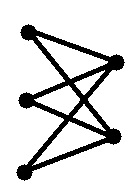
\includegraphics[width=0.25\textwidth]{figure2}
% 	\caption{Figure 2}
% \end{figure}

% \section{Draw the adjacency matrix $A$ for Figure 2}

% \[ \left( \begin{array}{ccccc}
% 0 & 1 & 0 & 1 & 0 \\
% 1 & 0 & 1 & 0 & 1 \\
% 0 & 1 & 0 & 1 & 0 \\
% 1 & 0 & 1 & 0 & 1 \\
% 0 & 1 & 0 & 1 & 0 \end{array} \right)\] 

% \section{Figure 2 Cycles} 
% \subsection{Amount of 2-cycles for the left-hand and right-hand vertices}

% \centerline{Left-hand: 6}
% \centerline{Right-Hand: 6}

% \subsection{Amount of 4-cycles for the left-hand and right-hand vertices} 

% \centerline{Left-hand: 6}
% \centerline{Right-Hand: 4}

% \subsection{Amount of 6-cycles for the left-hand and right-hand vertices} 

% \centerline{Left-hand: 0}
% \centerline{Right-Hand: 0}

\chapter{Design Goals}

	\section{Comparision of other Language Goals}

		Other programming languages have design goals. I'll probably use other languages as spring boards for my 
		relatively new language in terms of everything else.

	\section{Web Development}

\chapter{Syntax}

\section{C Language}

	Sprung from the Perl programming language. Oddly enough, with C++ as my first language I knew, it was easy for me to learn.

\chapter{Data Types}

\chapter{Data Structures}

\chapter{Conditionals}

	if
	if else
	elseif
	for loop
	while loop - pre checking
	do while - post checking

\chapter{Subprograms}

	Supports functions

\chapter{Data Abstractions}

\chapter{Parameter Passing}

\chapter{Concurrency}

\chapter{Recursion}

\chapter{Exception Handling}

\chapter{Expressions and Assignment Statements}

\chapter{Input/Output}

\chapter{Unusual Features}

\chapter{Contributions to the Programming Language Landscape}

\chapter{References}



\chapter{Personal Reflection}

	Consider the environment this programming language is being exposed to. Idiocy building on idiocy isn’t something you want, and is very hard to decipher between intelligence when surrounded by bad. I hesitate to fall head over heels in love with this language.

	People in the previous years had to wait a whole day for their code to compile. Waiting a whole day to find out there is a semi-colon missing provided incentive to pay attention to detail. JavaScript however is an interpreted language. This language’s interpreter is being supported by a majority of browsers being used by people today.

\end{document} 